\documentclass[12pt]{article}
%%---------------------------------------------------------------------
% packages
% geometry
\usepackage{geometry}
% font
\usepackage{fontspec}
\defaultfontfeatures{Mapping=tex-text}  %%如果没有它,会有一些 tex 特殊字符无法正常使用,比如连字符。
\usepackage{xunicode,xltxtra}
\usepackage[BoldFont,SlantFont,CJKnumber,CJKchecksingle]{xeCJK}  % \CJKnumber{12345}: 一万二千三百四十五
\usepackage{CJKfntef}  %%实现对汉字加点、下划线等。
\usepackage{pifont}  % \ding{}
% math
\usepackage{amsmath,amsfonts,amssymb}
% color
\usepackage{color}
\usepackage{xcolor}
\definecolor{EYE}{RGB}{199,237,204}
\definecolor{FLY}{RGB}{128,0,128}
\definecolor{ZHY}{RGB}{139,0,255}
% graphics
\usepackage[americaninductors,europeanresistors]{circuitikz}
\usepackage{tikz}
\usetikzlibrary{positioning,arrows,shadows,shapes,calc,mindmap,trees,backgrounds}  % placements=positioning
\usepackage{graphicx}  % \includegraphics[]{}
\usepackage{subfigure}  %%图形或表格并排排列
% table
\usepackage{colortbl,dcolumn}  %% 彩色表格
\usepackage{multirow}
\usepackage{multicol}
\usepackage{booktabs}
% code
\usepackage{fancyvrb}
\usepackage{listings}
% title
\usepackage{titlesec}
% head/foot
\usepackage{fancyhdr}
% ref
\usepackage{hyperref}
% pagecolor
\usepackage[pagecolor={EYE}]{pagecolor}
% tightly-packed lists
\usepackage{mdwlist}

\usepackage{styles/iplouccfg}
\usepackage{styles/zhfontcfg}
\usepackage{styles/iplouclistings}

%%---------------------------------------------------------------------
% settings
% geometry
\geometry{left=2cm,right=1cm,top=2cm,bottom=2cm}  %设置 上、左、下、右 页边距
\linespread{1.5} %行间距
% font
\setCJKmainfont{Adobe Kaiti Std}
%\setmainfont[BoldFont=Adobe Garamond Pro Bold]{Apple Garamond}  % 英文字体
%\setmainfont[BoldFont=Adobe Garamond Pro Bold,SmallCapsFont=Apple Garamond,SmallCapsFeatures={Scale=0.7}]{Apple Garamond}  %%苹果字体没有SmallCaps
\setCJKmonofont{Adobe Fangsong Std}
% graphics
\graphicspath{{figures/}}
\tikzset{
    % Define standard arrow tip
    >=stealth',
    % Define style for boxes
    punkt/.style={
           rectangle,
           rounded corners,
           draw=black, very thick,
           text width=6.5em,
           minimum height=2em,
           text centered},
    % Define arrow style
    pil/.style={
           ->,
           thick,
           shorten <=2pt,
           shorten >=2pt,},
    % Define style for FlyZhyBall
    FlyZhyBall/.style={
      circle,
      minimum size=6mm,
      inner sep=0.5pt,
      ball color=red!50!blue,
      text=white,},
    % Define style for FlyZhyRectangle
    FlyZhyRectangle/.style={
      rectangle,
      rounded corners,
      minimum size=6mm,
      ball color=red!50!blue,
      text=white,},
    % Define style for zhyfly
    zhyfly/.style={
      rectangle,
      rounded corners,
      minimum size=6mm,
      ball color=red!25!blue,
      text=white,},
    % Define style for new rectangle
    nrectangle/.style={
      rectangle,
      draw=#1!50,
      fill=#1!20,
      minimum size=5mm,
      inner sep=0.1pt,}
}
\ctikzset{
  bipoles/length=.8cm
}
% code
\lstnewenvironment{VHDLcode}[1][]{%
  \lstset{
    basicstyle=\footnotesize\ttfamily\color{black},%
    columns=flexible,%
    framexleftmargin=.7mm,frame=shadowbox,%
    rulesepcolor=\color{blue},%
%    frame=single,%
    backgroundcolor=\color{yellow!20},%
    xleftmargin=1.2\fboxsep,%
    xrightmargin=.7\fboxsep,%
    numbers=left,numberstyle=\tiny\color{blue},%
    numberblanklines=false,numbersep=7pt,%
    language=VHDL%
    }\lstset{#1}}{}
\lstnewenvironment{VHDLmiddle}[1][]{%
  \lstset{
    basicstyle=\scriptsize\ttfamily\color{black},%
    columns=flexible,%
    framexleftmargin=.7mm,frame=shadowbox,%
    rulesepcolor=\color{blue},%
%    frame=single,%
    backgroundcolor=\color{yellow!20},%
    xleftmargin=1.2\fboxsep,%
    xrightmargin=.7\fboxsep,%
    numbers=left,numberstyle=\tiny\color{blue},%
    numberblanklines=false,numbersep=7pt,%
    language=VHDL%
    }\lstset{#1}}{}
\lstnewenvironment{VHDLsmall}[1][]{%
  \lstset{
    basicstyle=\tiny\ttfamily\color{black},%
    columns=flexible,%
    framexleftmargin=.7mm,frame=shadowbox,%
    rulesepcolor=\color{blue},%
%    frame=single,%
    backgroundcolor=\color{yellow!20},%
    xleftmargin=1.2\fboxsep,%
    xrightmargin=.7\fboxsep,%
    numbers=left,numberstyle=\tiny\color{blue},%
    numberblanklines=false,numbersep=7pt,%
    language=VHDL%
    }\lstset{#1}}{}
% pdf
\hypersetup{pdfpagemode=FullScreen,%
            pdfauthor={Haiyong Zheng},%
            pdftitle={Title},%
            CJKbookmarks=true,%
            bookmarksnumbered=true,%
            bookmarksopen=false,%
            plainpages=false,%
            colorlinks=true,%
            citecolor=green,%
            filecolor=magenta,%
            linkcolor=cyan,%red(default)
            urlcolor=cyan}
% section
%http://tex.stackexchange.com/questions/34288/how-to-place-a-shaded-box-around-a-section-label-and-name
\newcommand\titlebar{%
\tikz[baseline,trim left=3.1cm,trim right=3cm] {
    \fill [cyan!25] (2.5cm,-1ex) rectangle (\textwidth+3.1cm,2.5ex);
    \node [
        fill=cyan!60!white,
        anchor= base east,
        rounded rectangle,
        minimum height=3.5ex] at (3cm,0) {
        \textbf{\thesection.}
    };
}%
}
\titleformat{\section}{\Large\bf\color{blue}}{\titlebar}{0.1cm}{}
% head/foot
\setlength{\headheight}{15pt}
\pagestyle{fancy}
\fancyhf{}
%\lhead{\color{black!50!green}2014年秋季学期}
\chead{\color{black!50!green}显著性检测}
%\rhead{\color{black!50!green}通信电子电路}
\lfoot{\color{blue!50!green}朱亚菲}
\cfoot{\color{blue!50!green}\href{http://vision.ouc.edu.cn/~zhenghaiyong}{CVBIOUC}}
\rfoot{\color{blue!50!green}$\cdot$\ \thepage\ $\cdot$}
\renewcommand{\headrulewidth}{0.4pt}
\renewcommand{\footrulewidth}{0.4pt}


%%---------------------------------------------------------------------
\begin{document}
%%---------------------------------------------------------------------
%%---------------------------------------------------------------------
% \titlepage
\title{\vspace{-2em}显著性检测\vspace{-0.7em}}
\author{朱亚菲}
\date{\vspace{-0.7em}2015年2月\vspace{-0.7em}}
%%---------------------------------------------------------------------
\maketitle\thispagestyle{fancy}
%%---------------------------------------------------------------------
\maketitle
\tableofcontents 

\section{引言}

由论文“A closer look at context: from coxes to the contextual emergence of object saliency”知道


\section{多尺度的概念}

多尺度

\section{Hierarchical Saliency Detection}

这篇论文主要解决的是当图像中显著前景或背景中存在小尺度大对比度patterns,而在生成的显著图中并不突出这些patterns的情况。论文框架如图~\ref{fig: hsaliency1}。主要步骤是三步:首先从原图像中提取layers,然后从每个layer中计算saliency cues,最后把它们融入一个分层模型以得到最终的结果。

\begin{figure}[!ht]
\centering
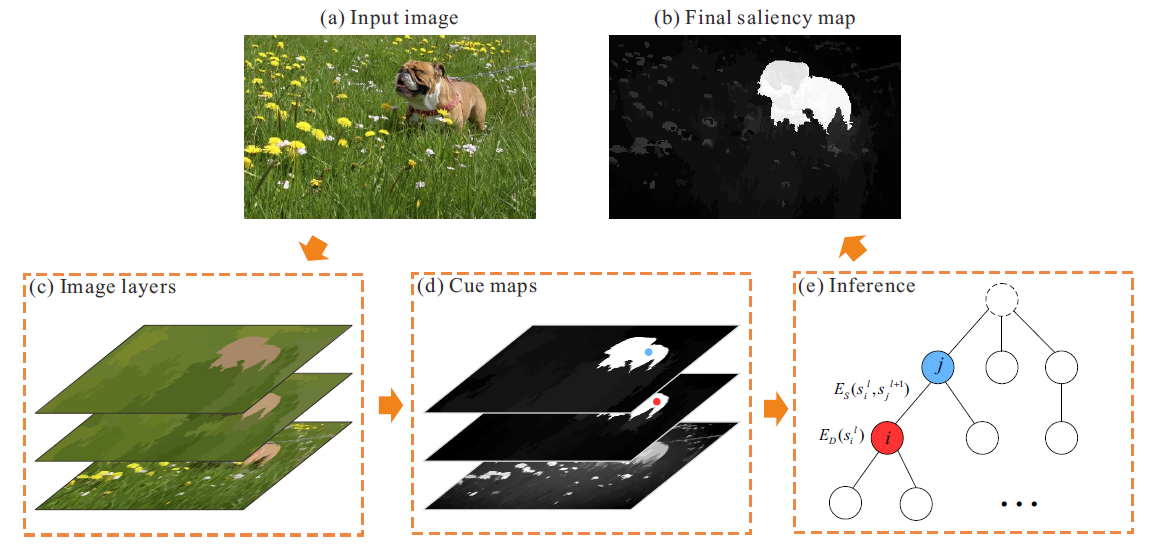
\includegraphics[width=0.8\textwidth]{hsaliency1.png}
\caption{框架}
\label{fig: hsaliency1}
\end{figure} 

分层与多尺度、多分辨率的区别?

1. 如何提取这三个layers?如图~\ref{fig: hsaliency2}

\begin{figure}[!ht]
\centering
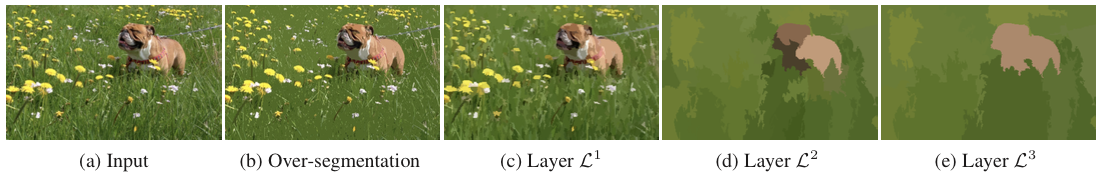
\includegraphics[width=0.85\textwidth]{hsaliency2.png}
\caption{不同尺度下的区域合并结果}
\label{fig: hsaliency2}
\end{figure}

先对原图像($400 \times 300$)用watershed-like方法~\cite{gonzalez2009digital}进行初始的过分割,对每个分割区域计算一个scale值,然后对所有区域的scale值按从小到大排序,如果一个区域的scale值小于3,就将它和最近的区域合并(通过判断两个区域内CIELUV颜色均值的距离),然后更新它的scale,并更新合并区域的颜色均值,等对所有区域都处理后,得到的结果就是$L^1$层。$L^2$层是通过对$L^1$层采取同样的步骤,只不过用一个更大的阈值17。$L^3$层也是如此,阈值取33。

2. 如何求每个区域的scale?

通常在Mean shift、graph-based segmentation等超像素分割方法中,区域的size是指该区域内所有像素的个数。本论文指出了这样的不合理性,就人类视觉感知而言,较多的像素个数和大尺度的区域并不完全符合。如图~\ref{fig: hsaliency3},尽管弯曲的区域a包含了很多像素,但对于我们的视觉感受却并不觉得它很大,而b看着会更大一些,尽管它的像素个数并不是很多。根据这样的现象,作者基于shape uniformities定义了一个新的encompassment scale measure,以用来在合并阶段获取区域的size。

\begin{figure}[!ht]
\centering
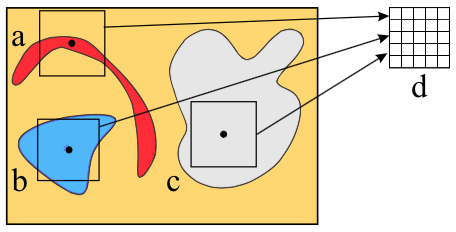
\includegraphics[width=0.4\textwidth]{hsaliency3.png}
\caption{scale}
\label{fig: hsaliency3}
\end{figure}

关于scale的定义如下:
\begin{align}
scale(R) == arg \max_i {R_{t \times t}|R_{t \times t} \subseteq R}
\end{align}

其中,$R_{t \times t}$是一个$t \times t$的正方形区域。也就是说,一个区域的scale是指该区域内所能包含的最大方形区域的边长。这里并不需要通过复杂的计算来算出每个区域的scale是多大,只要判断其相对于阈值是大还是小,这样就简化了,可以对每个区域用一个$t \times t$的模板进行滤波,如果滤完后该区域内所有像素值都被更新了,说明该区域的scale小于t,反之说明大于t,如图~\ref{fig: hsaliency4}所示。

\begin{figure}[!ht]
\centering
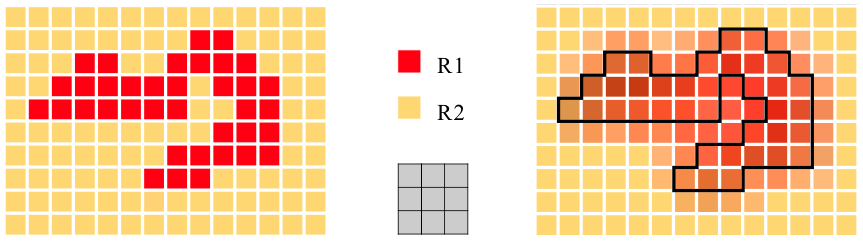
\includegraphics[width=0.6\textwidth]{hsaliency4.png}
\caption{scale}
\label{fig: hsaliency4}
\end{figure}

3. 如何计算每一层的saliency cues?

主要从颜色、位置、大小三个方面提取saliency cues,以找到该层比较重要的pixels,作者用了两种cues:

1)local contrast

\begin{align}
C_i = \sum_{j=1}^{n}w(R_i)\Phi(i, j)||c_i-c_j||_2
\end{align}
其中$c_i$和$c_j$分别表示区域$R_i$和$R_j$中的颜色,$w(R_j)$指$R_j$中像素的个数。$\Phi(i, j) = exp\{-D(R_i, R_j)/\sigma^2\}$,控制了区域$R_i$和$R_j$之间的空间距离,其中$D(R_i, R_j)$是区域$R_i$和$R_j$的中心的欧几里得距离的平方。

2)location heuristic

心理物理学方面的研究表示人类视觉注意偏好图像的中央区域,所以在通常情况下越靠近图像中央的像素越显著。
\begin{align}
H_i = \frac{1}{w(R_i)}\sum_{x_i \in R_i} exp\{-\lambda||x_i-x_c||^2\}
\end{align}
其中$\{x_0, x_1\ldots\}$是区域$R_i$中的像素坐标的集合,$x_c$是图像中心坐标。

然后将$C_i$与$H_i$组合起来,得到
\begin{align}
\bar{s}_i = C_i \cdot H_i
\end{align}

由于local contrast和location cues都被归一化到$[0, 1)$,它们各自的重要性由$\lambda$来控制。当对三个layers均计算完$\bar{s}_i$后,就可以得到每一层的初始显著图,最后通过一种hierarchical inference procedure来对多尺度显著性检测结果进行融合。

4. 最后一步Hierarchical Inference是怎么进行的?

Cue maps显示了不同尺度下的显著性,效果很不一样。在底层,会产生很多小区域,而在高层会包含大尺度的结构。由于图像的多样性,单独的一层并不能保证效果是完美的,也很难判别哪一层是效果最好的。

由于背景或前景的复杂性,单纯通过求这三层产生的显著图的平均值来融合并不是一个好的选择。作者构造了一个基于树结构的图,见图~\ref{fig: hsaliency1}中的(e),其中的节点代表相应层中的区域。节点$j$在下一层中包含两个分割区域,因而有两个子节点。其中父节点代表整幅图像的最粗糙表示。

将图中对应于第$L_l$层中第$i$个区域的节点上的显著性定义为变量$s_i^l$,设$S$是包含图中所有节点的集合。最小化如下的能量方程:
\begin{align}
E(S) = \sum_l \sum_i E_D(s_i^l)+\sum_l \sum_{i, R_i^l \subseteq R_j ^{l+1}} E_S(s_i^l, s_j^{l+1})
\end{align}

\section{2014CVPR-LuSong-Learning optimal seeds for diffusion-based salient objectt detection}

\section{2013CVPR-MaiLong-Saliency Aggregation: A Data-driven Approach}

方法动机:目前在视觉显著性分析方面有很多的方法,每种方法可能对某一些图像或图像中的某些部分适用,能产生较好的结果,却没有哪一种方法能对所有的图像都适用。并且不同的显著性计算方法之间通常是互补的。因而可以尝试对这些显著性计算方法进行组合以获得比使用单一的一种方法好的效果。一般的融合方法都是预先定义好一个组合方程,并且其中每种方法的重要程度都是一样的。而论文中采用的是CRF aggregation框架来进行显著性聚合,不仅考虑了各个显著图的贡献,还考虑了相邻像素间的相互作用。由于每种方法在不同图像上的表现也不同,所以对每幅图像使用的方法组合也是不同的。考虑到每幅图像上聚合的依赖性,该方法首先从训练数据集中选择与输入图像近似的图像子集,以在这个子集上而不是在整个训练集上训练这个CRF aggregation model。

该方法有以下两点优势:

1. 考虑了不同显著性方法的性能gaps,可以更好地决定每种方法在融合时的贡献大小。

2. 考虑到各个显著性方法在处理不同图像时效果有所不同,该方法能对不同图像自适应选择合适的融合model。

步骤如下:

对给定的图像$I$,首先运行$m$种显著性方法$\{M_i||1\le i\le m\}$,以产生$m$幅显著图$\{S_i||1\le i\le m\}$。显著图中的每个元素$S_i(p)$代表了像素点$p$处的显著值。显著图中的显著值都被归一化到$[0, 1]$。输入这$m$幅显著图,输出最终的显著图$S$。

\section{Saliency Detection via Graph-Based Manifold Ranking}

方法动机:以往的显著性检测方法大多是通过计算某像素或区域在局部的上下文中或整幅图像中的对比度来得到该像素或区域上的显著性值,这篇论文则是通过计算图像元素(像素或区域)和foreground cues以及background cues的相似度来得到该图像元素上的显著度,相似度是通过graph-based manifold ranking求得的。

background cue:背景通常与图像的四个边界呈现局部或整体上的外观关联性

foreground cue:foreground presents appearance coherence and consistency

算法步骤如图~\ref{fig: MR1},先对图像进行超像素分割,然后将分割后的图像映射为图,每个超像素为图中的节点。第一个阶段是将图像的每一条边界上(共4条)的节点看作是labelled background queries,依次算图中的每个节点与这些queries的相关性来得到4幅labelled maps,然后对其进行融合得到显著图。在第二阶段,对第一阶段得到的显著图二值化,然后将得到的labelled foreground节点看作是salient queries,最终每个节点的显著度就是通过计算其与foreground queries的相关性得到。
\begin{figure}[!ht]
\centering
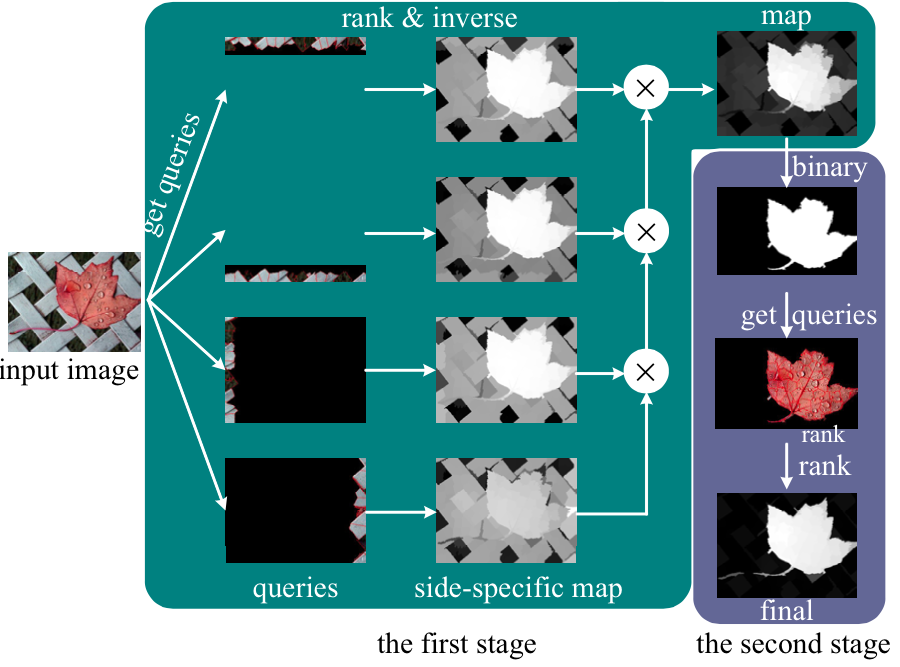
\includegraphics[width=0.7\textwidth]{MR1.png}
\caption{算法步骤}
\label{fig: MR1}
\end{figure}

第一阶段与第二阶段中的ranking function是什么呢?

\section{Saliency Optimization from Robust Background Detection}

这个论文是基于假设:an image patch is background only when the region it belongs to is heavily connected to the image boundary.

动机:目前虽然已有方法利用了boundary prior,但一般是基于假设:将图像边缘区域看作是背景。这些方法有两方面的缺点:一是当目标物体稍微接触图像边缘时,效果就会变差。二是它们只是探索性的,并没有告诉我们怎样将其跟其他saliency cues相融合。

这篇论文主要有两个方面的贡献:

1. 提出了一种非常鲁棒的boundary connectivity方法

2. 提出了融合多种low level cues的优化框架

关于boundary connectivity的一个示例:
\begin{figure}[!ht]
\centering
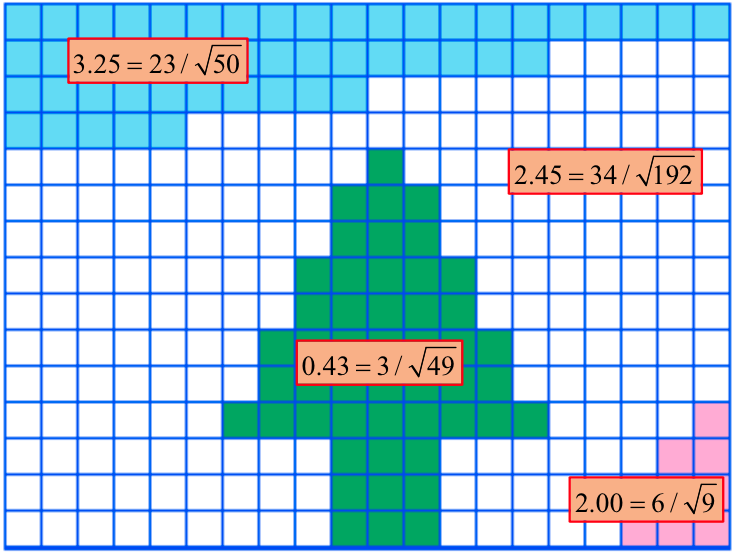
\includegraphics[width=0.5\textwidth]{wCtr.png}
\caption{关于boundary connectivity的一个图例}
\label{fig: wCtr}
\end{figure}

图~\ref{fig: wCtr}是一幅人造图,共有四个区域。对于人类的视觉感知来说,图中绿色的区域很显然是显著区域,因为它满足以下条件:大、紧凑、仅仅轻微地接触图像边缘。粉色区域与图像边缘接触也很少,但它的size太小了,使得它更像是一个被部分切断了的物体,因而不是显著的。基于此,论文中提出了一种方法来将区域$R$与图像边缘的连接程度量化,叫做boundary connectivity,定义如下:
\begin{align}
BndCon(R) = \frac{|\{p|p \in R, p \in Bnd\}|}{\sqrt{|\{p|p \in R\}|}}
\end{align},
其中$Bnd$是处于图像边缘的图像块的集合,$p$是图像块。该公式在几何上的解释是:它是一个区域在边缘上的perimeter与该区域的整个perimeter的比值。这里用的是区域面积的平方根,目的是保持尺度不变性:在不同resolution的图像块上的效果保持稳定。如图~\ref{fig: wCtr}所示,对于背景区域,boundary connectivity值通常较大,而对目标区域,boundary connectivity值通常较小。

有了boundary connectivity的定义,要计算它的值仍然是比较困难的,因为图像分割本身就是一个复杂的问题。用像图~\ref{fig: wCtr}中的hard segmentation不仅会涉及分割方法选择的难题,而且会在区域边界产生不想要的间断性。

论文中指出精确的hard image segmentation是没有必要的,只需要用一种“soft”的分割方法。

论文的基本步骤如下:

1. 用SLIC方法将图像先分割成超像素,対一幅$300 \times 400$的图像,取超像素个数为200个足够了。

2. 构造无向图,超像素作为节点,相邻的超像素之间连成边,边的权值用两个超像素区域在CIE-Lab颜色空间上的颜色均值的欧几里得距离$d_{app}(p, q)$表示。

两个超像素之间的deodesic distance被定义为它们在图上最短路径的累计权值和:
\begin{align}
d_{geo}(p, q) = \min_{p_1=p, p_2, \ldots, p_n=q}\sum_{i=1}^{n-1}d_{app}(p_i, p_{i+1})
\end{align}

为方便体现,定义$d_{geo}(p, p) = 0$。每个超像素$p$的spanning area定义为:
\begin{align}
Area(p) = \sum_{i=1}^N exp(-\frac{d_{geo}^2(p, p_i)}{2\sigma_{clr}^2})=\sum_{i=1}^N S(p, p_i)
\end{align}

其中,$N$是超像素的个数。可以看到,$S(p, p_i)$的范围一直在$(0, 1]$之间,并且表征了超像素$p_i$对$p$的贡献大小。当$p_i$和$p$在一个较平坦的区域内,则有$d_{geo}(p, p_i) = 0$,并且$S(p, p_i) =1$,保证$p_i$对区域$p$增加了一个单位区域。而当$p_i$和$p$在不同的区域中时,它们的最短路径中至少有一个边满足$d_{app}(*, *)\ge 3\sigma_{clr})$,使得$S(p, p_i)\approx0$,保证$p_i$不对$p$的area产生影响。通过实验发现参数$\sigma_{clr}$在$[5,15]$之间时效果是稳定的,在作者试验中取$\sigma_{clr}=10$。

同样地,将length along the boundary定义为:
\begin{align}
Len_{bnd}(p) = \sum_{i=1}^N S(p, p_i) \cdot \delta(p_i \in Bnd)
\end{align}

最后,计算boundary connectivity
\begin{align}
BndCon(p) = \frac{Len_{bnd}(p)}{\sqrt{Area(p)}}
\end{align}

到这里,只是计算出了某区域的boundary connectivity值,还没有求出最终的显著图。以前的显著性方法通常将某区域和周围区域之间的region contrast看成一种saliency cue,计算如下:
\begin{align}
Ctr(p) = \sum_{i=1}^{N}d_{app}(p, p_i)w_{spa}(p, p_i),
\end{align}
其中,$d_{app}(p, p_i)$是两个区域在CIELab空间上的颜色均值的欧几里得距离,$w_{spa}(p, p_i)$是区域之间的空间距离,$w_{spa}(p, p_i) = exp(-\frac{d_{spa}^2(p, p_i)}{2\sigma_{spa}^2})$,$d_{spa}(p, p_i)$是超像素$p$和$p_i$的中心间的距离,$\sigma_{spa}$取0.25。

论文中对上述方程进行了扩展,加入了一项新的权重项背景概率$w_i^{bg}$。$w_i^{bg}$是从超像素的boundary connectivity值映射来的。当boundary connectivity值较大时,$w_i^{bg}$接近1,当boundary connectivity值较小时,$w_i^{bg}$接近。定义如下:
\begin{align}
w_i^{bg} = 1-exp(-\frac{BndCon^2(p_i)}{2\sigma_{bndCon}^2}),
\end{align}
这里令$\sigma_{bndCon}=1$。

于是扩展后的contrast公式如下:
\begin{align}
wCtr(p) = \sum_{i=1}^{N}d_{app}(p, p_I)w_{spa}(p, p_i)w_i^{bg},
\end{align}
当$p$是背景区域时,$wCtr(p)$是与其相邻的目标区域的背景关联度的加权,值较小;当$p$是目标区域时,$wCtr(p)$是与其相邻的背景区域的背景关联度的加权,值较大。满足对显著性的定义。

全局优化:定义cost function如下
\begin{align}
\sum_{i=1}^{N}w_i^{bg}s_i^2+\sum_{i=1}^{N}s_i^{fg}(s_i-1)^2+\sum_{i, j}w_{ij}(s_i-s_j)^2,
\end{align}
其中第一项是背景约束,当某区域的$w_i^{bg}$较大时,是背景的概率较大,方程的第一项占的比重较多,为使整个方程值最小,需使$s_i$近似为0,也就是使该区域的显著性近似为0。第二项是前景约束,当某区域的$w_i^{fg}$较大时,第二项占的比重较大,需使$s_i$近似为1。$w_i^{fg}$可以通过目前已有的一些显著性方法或它们的组合来计算。第三项是平滑约束,保证显著值的连续性,$w_{ij}$定义如下:
\begin{align}
w_{ij} = exp(-\frac{d_{app}^2(p_i, p_j)}{2\sigma_{clr}^2})+\mu
\end{align}
超像素$p_i$与$p_j$越相似,$d_{app}(p_i, p_j)$越小,$w_{ij} $越大,越需要$s_i$,$s_j$近似相等。

\section{Graph-Regularized Saliency Detection With Convex-Hull-Based Center Prior}

简称PBS(the proposed prior based saliency)~\cite{yang2013graph}。

文章动机:Center prior虽然被广泛用到了显著性检测方法中,但是它还有一定的缺陷。比如在很多图像中,显著物体可能会出现在偏离图像中心的位置,这就使得在用center prior时会错误地抑制掉离图像中心很远的目标区域而将靠近图像图像中心的背景区域高亮显示。另外之前的一些方法在计算每个像素点或区域的显著值时是各自独立的,而忽略了相似像素点上显著性值应该近似的现象。基于这两个方面,文章中引入了convex-hull-based center prior和smoothness prior。

算法步骤:

1. 先将给定图像用SLIC方法分割成超像素。

2. 计算初始显著图。先计算了spatially weighted contrast
\begin{align}
S_{co}(i) = \sum_{j \ne i}||c_i-c_j|| \cdot exp\left(-\frac{||p_i-p_j||^2}{2\sigma_p^2}\right)
\end{align}
然后又计算了convex-hull-based center prior map,即首先估计显著目标的中心位置$(x_0, y_0)$,再计算每个超像素$i$的显著性:
\begin{align}
S_{ce}(i) = exp\left(-\frac{||x_i-x_0||^2}{2\sigma_x^2}-\frac{||y_i-y_0||^2}{2\sigma_y^2}\right)
\end{align}
最后将两者相乘得到初始显著图
\begin{align}
S_{in}(i) = S_{co}(i) \times S_{ce}(i)
\end{align}

使用convex-hull-based center prior后虽然会改善当显著目标偏离图像中心的情况,但仍然存在以下局限性:1. convex-hull-based center prior的效果取决于所求convex hull的精确度。2. 由于取$\sigma_x$和$\sigma_y$相等并且固定,所以当显著目标不是对称的并且大小是随图像不同而变化的时候,会导致初始显著图的不准确性。

引入smoothness prior可以解决这一问题,得到更精细的显著图。平滑约束通常是用在基于图的目标分割中,目的是使图像中相邻的像素拥有同样的label值。论文中先将图像分割成超像素,然后将其映射为图,每个超像素对应图中的节点,有共同的边界的超像素之间有一条边,边上的权值为$w_{ij} \in W$:
\begin{align}
w_{ij} = exp\left(-\frac{||c_i-c_j||}{2\sigma_w^2}\right),
\end{align}
其中$c_i$和$c_j$是CIELab空间超像素区域内像素的颜色均值。可以看到关系矩阵$W$是一个稀疏矩阵。定义如下saliency cost function来表示这种smoothness prior:
\begin{align}
E(S) = \sum_i(S(i)-S_{in}(i))^2+\lambda\sum_{i,j}w_{ij}(S(i)-S(j))^2
\end{align}
$S(i)$和$S(i)$分别表示节点$i$和$j$的所要求的显著值,$S_{in}(i)$是节点$i$的初始显著值,$\lambda$是规范化系数。其中等式右边第一项是fitting constraint,表示一幅好的显著图与初始显著图之间不会变化太多。第二项是smoothness constraint,一幅好的显著图上相邻超像素的显著值不会相差太多。超像素上的最优显著值是通过最小化该cost function来计算。令该方程关于$S$的导数为0可得
\begin{align}
S^* = \mu (D-W+\mu I)^{-1}S_{in}
\end{align}
其中$D$是三角矩阵,并且有$d_{ii} = \sum_j (w_{ij})$,$\mu = 1/(2\lambda)$。

\section{Saliency Detection via Absorbing Markov Chain}

马尔可夫链,因安德烈$\cdot$马尔可夫(A.A.Markov, 1856-1922)得名,是数学中具有马尔可夫性质的离散事件随机过程。该过程中,在给定当前知识或信息的情况下,只有当前的状态用来预测将来,过去(即当前以前的历史状态)对于预测将来(即当前以后的未来状态)是无关的。

$X_1, X_2, X_3\ldots$马尔可夫链(Markov Chain),描述了一种状态序列,其每个状态值取决于前面有限个状态。马尔可夫链是具有马尔可夫性质的随机变量的一个数列。这些变量的范围,即它们所有可能取值的集合,被称为“状态空间”,而$X_n$的值则是在时间$n$的状态。如果$X_{n+1}$对于过去状态的条件概率分布仅是$X_n$的一个函数,则
\begin{align}
P(X_{n+1}=x|X_1=x_1, X_2=x_2, \ldots, X_n=x_n)=P(X_{n+1}=x|X_n=x_n)
\end{align}
这里$x$为过程中的某个状态。上面这个恒等式可以被看作是马尔可夫性质。

在马尔可夫链的每一步,系统根据概率分布,可以从一个状态变到另一个状态,也可以保持当前状态。状态的改变叫做过渡,与不同的状态改变相关的概率叫做过渡概率。随机游走就是马尔可夫链的例子。随机游走中每一步的状态是在图形中的点,每一步可以移动到任何一个相邻的点,在这里移动到每一个点的概率都是相同的(无论之前漫步路径是如何的)。

在马尔可夫链中,称$P_{ij}=1$的状态为吸收状态。如果一个马尔科夫链中至少包含一个吸收状态,并且从每一个非吸收状态出发,都可以到达某个吸收状态,那么这个马尔可夫链称为吸收马尔可夫链(Absorbing Markov Chains)。如图~\ref{fig: Drunkard-Walk},这是一个醉汉游走模型,当醉汉处于位置1、2或者3时,他将会以等概率(1/2)向左或者向右走,他一直走,直到他到达位置0(他的家)或者位置4(酒吧)才停止游走。
\begin{figure}[!ht]
\centering
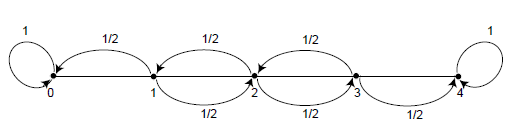
\includegraphics[width=0.7\textwidth]{Drunkard-Walk.png}
\caption{Drunkard's Walk}
\label{fig: Drunkard-Walk}
\end{figure}






















%
% references
\bibliographystyle{plain}

\bibliography{saliency} %参考文献


\end{document}